\documentclass[11pt]{article}

\usepackage[margin=1in]{geometry}
\usepackage{amsmath, amssymb, amsfonts}
\usepackage{booktabs}
\usepackage{graphicx}
\usepackage{float}
\graphicspath{{figures/}{lqr-lqi-learning-curves/figures/}}
\usepackage[colorlinks=true, linkcolor=blue, urlcolor=blue, citecolor=blue]{hyperref}

\title{Notes: Measuring Reinforcement Learning Against the Exact LQR Optimum}
\author{Jon Legasa}
\date{\today}

\begin{document}

\maketitle

\section*{Summary}

LQR has become a standard for measuring RL algorithms, but we found that some algorithms have not
been tested on it, and we are trying to see the impact of LQR across many seeds to see the behavior
of these algorithms. We seek to understand whether there is any way to measure the performance of
these algorithms with respect to each other, and then to measure their performance on RL
environments to see if these differences in performance hold even for many seeds.

%----------------------------------------------------------------------------------------------------
\section{Motivation}

We came together to try to find what makes these algorithms special, following consistent
benchmarks and baselines. We set up the LQR step to motivate the baseline (Section~\ref{sec:riccati}).
Agyei, Sarhadi and Polani (2025) introduced LQI as the baseline for comparing deep RL algorithms on
tracking problems in continuous time, one of them nonlinear (Section~\ref{sec:lqi}). From this
baseline we extend to those setups.

We then introduce the many seeds, the expected value and the average of the learning curves
(Section~\ref{sec:seeds}), because we expect the learning curves to converge to the same value
across seeds, and to be bounded. Think of the set of seeds as points on a line, any of which can be
picked. As we observe all seeds and measure the performance of every algorithm, it could be possible
that, as training time increases, for all seeds on this line the algorithms generate learning curves
that satisfy an ordering inequality. That is the setup of these notes.

The LQR is a standard diagnostic for RL because its optimal controller is known (Recht 2019).
Earlier LQR comparisons covered certainty equivalence, least-squares policy iteration, REINFORCE and
random search (Recht 2019; Mania, Guy and Recht 2018). Agyei et al.\ compared deep RL methods with an
LQI controller using step-response metrics.

%----------------------------------------------------------------------------------------------------
\section{Problem and notation}
\label{sec:problem}

\[
  x_{t+1} = A x_t + B u_t, \qquad c(x, u) = x^\top Q x + u^\top R u, \qquad
  J(\pi) = \sum_{t=0}^{\infty} c(x_t, u_t).
\]

Here $x_t$ is the state at time $t$ and $u_t$ is the control; $A$ describes how the state evolves on
its own and $B$ how the control acts on it. The \textbf{stage cost} is the cost paid at time $t$:
\[
  c(x_t, u_t) = \underbrace{x_t^\top Q\, x_t}_{\text{distance from } 0}
  + \underbrace{u_t^\top R\, u_t}_{\text{control effort}},
  \qquad Q \succeq 0, \quad R \succ 0 .
\]
In the scalar case, $A$, $B$, $Q$ and $R$ are the numbers $a$, $b$, $q$ and $r$.

$J(\pi)$ is the total cost of following the policy $\pi$ from $x_0$: run the system under $\pi$ and
add up the stage costs. The system is noise-free and undiscounted, with fixed $x_0$
(Section~\ref{sec:limitations} covers noise and discounting). Policies are linear, $u = -Kx$, and
$J^* = \min_\pi J(\pi)$ is attained at $K^*$, as derived in Section~\ref{sec:riccati}. The agent
receives the reward $r_t = -c(x_t, u_t)$ and does not know $A$, $B$, $Q$, $R$, $K^*$ or $J^*$; these
are used only to evaluate it. Algorithms $A$, $B$ and $C$ (PPO, SAC and TD3) are trained with many
seeds, and $N$ counts training iterations.

%----------------------------------------------------------------------------------------------------
\section{The Riccati solution}
\label{sec:riccati}

The Riccati equation is the Bellman equation of the LQR, reduced to an equation for a single
matrix. The optimal cost-to-go $V(x)$, the total cost of acting optimally from state $x$, satisfies
\[
  V(x) = \min_u \Big[\, x^\top Q x + u^\top R u + V(A x + B u) \,\Big].
\]

Guess that the cost-to-go is quadratic, with a symmetric positive semidefinite matrix $P$; the guess
is confirmed if it leads to a consistent equation for $P$. Substituting it, the bracket becomes
\[
  V(x) = x^\top P x, \qquad x^\top Q x + u^\top R u + (A x + B u)^\top P (A x + B u).
\]
This is a convex quadratic in the control, because $R$ is positive definite and the term with $P$ is
positive semidefinite. Its gradient with respect to the control is
\[
  \nabla_u = 2 R u + 2 B^\top P (A x + B u) = 2\big(R + B^\top P B\big) u + 2 B^\top P A\, x ,
\]
and setting it to zero gives the optimal control:
\[
  u^* = -\big(R + B^\top P B\big)^{-1} B^\top P A\, x = -K^* x .
\]

Substituting the optimal control back, both sides of the Bellman equation are quadratic forms in
the state:
\[
  x^\top P x = x^\top \Big[\, Q + K^{*\top} R K^* + (A - B K^*)^\top P (A - B K^*) \,\Big] x .
\]
Expanding the last term and grouping the two terms that contain the gain twice:
\[
  Q + A^\top P A - A^\top P B K^* - K^{*\top} B^\top P A + K^{*\top} \big(R + B^\top P B\big) K^* .
\]
The definition of the optimal gain gives the identity below, which makes the last term equal to the
one before it, so those two cancel:
\[
  \big(R + B^\top P B\big) K^* = B^\top P A
  \quad\Longrightarrow\quad
  K^{*\top} \big(R + B^\top P B\big) K^* = K^{*\top} B^\top P A .
\]
What remains is the matrix in brackets, and it must equal $P$ because the two quadratic forms agree
for every state and both matrices are symmetric. This is the discrete algebraic Riccati equation,
shown with the optimal gain and the optimal cost:
\begin{gather*}
  P = Q + A^\top P A - A^\top P B \big(R + B^\top P B\big)^{-1} B^\top P A, \\
  K^* = \big(R + B^\top P B\big)^{-1} B^\top P A, \qquad J^* = x_0^\top P x_0 .
\end{gather*}

$P$ is the cost-to-go matrix: the optimal cost is the cost-to-go at the initial state, which is why
the optimal cost is the quadratic form of $P$ at the initial state. The equation is algebraic
because, over an infinite horizon, $P$ does not change with time; it is a fixed point of the Bellman
equation. It is quadratic in $P$.

\paragraph{The scalar case.} With $n = m = 1$:
\[
  A = [a], \quad B = [b], \quad Q = [q], \quad R = [r], \quad P = [p].
\]
Substituting term by term into the Riccati equation, with transposes acting trivially on numbers:
\[
  P = Q + \underbrace{A^\top P A}_{(1)} - \underbrace{A^\top P B}_{(2)}\,
  \underbrace{\big(R + B^\top P B\big)^{-1}}_{(3)}\, \underbrace{B^\top P A}_{(4)},
\]
\begin{align*}
  (1)\;& A^\top P A = a\, p\, a = a^2 p, &
  (2)\;& A^\top P B = a\, p\, b = a b\, p, \\
  (3)\;& \big(R + B^\top P B\big)^{-1} = \frac{1}{r + b\, p\, b} = \frac{1}{r + b^2 p}, &
  (4)\;& B^\top P A = b\, p\, a = a b\, p .
\end{align*}
Multiplying (2), (3) and (4) gives the scalar Riccati equation:
\[
  (2)(3)(4) = a b\, p \cdot \frac{1}{r + b^2 p} \cdot a b\, p = \frac{a^2 b^2 p^2}{r + b^2 p},
  \qquad
  p = q + a^2 p - \frac{a^2 b^2 p^2}{r + b^2 p} .
\]
With $a = b = q = r = 1$ and $x_0 = 1$, taking the root with $p \ge 0$:
\[
  p = 1 + p - \frac{p^2}{1 + p}
  \ \Longrightarrow\ 0 = 1 - \frac{p^2}{1 + p}
  \ \Longrightarrow\ p^2 = 1 + p
  \ \Longrightarrow\ p^2 - p - 1 = 0
  \ \Longrightarrow\ p = \frac{1 + \sqrt{5}}{2},
\]
\[
  K^* = \frac{a b\, p}{r + b^2 p} = \frac{p}{1 + p} = \frac{\sqrt{5} - 1}{2} \approx 0.618,
  \qquad
  J^* = p\, x_0^2 = \frac{1 + \sqrt{5}}{2} \approx 1.618 .
\]

So the cost-to-go matrix is the $1 \times 1$ matrix $[p]$, and $V(x) = p x^2$. Note
$(K^*)^2 + K^* - 1 = 0$ and $K^* J^* = 1$. In higher dimensions $P$ stays a genuine matrix, and the
Riccati equation is a system of coupled quadratic equations in its entries, usually solved
numerically.

%----------------------------------------------------------------------------------------------------
\section{From LQR to LQI}
\label{sec:lqi}

LQR drives the state to zero. A tracking problem asks an output to follow a reference instead, and
with a constant disturbance LQR leaves a permanent error. LQI is LQR applied to a system enlarged by
one state that accumulates the error.

\paragraph{The offset under a constant disturbance.} Add a constant disturbance to the system and
apply the LQR controller:
\[
  x_{t+1} = A x_t + B u_t + d, \qquad u_t = -K x_t .
\]
At steady state the state stops changing, so it must satisfy
\[
  x_{\mathrm{ss}} = (A - B K)\, x_{\mathrm{ss}} + d
  \quad\Longrightarrow\quad
  x_{\mathrm{ss}} = \big(I - A + B K\big)^{-1} d \neq 0 .
\]
In the scalar example the steady state is a multiple of the disturbance:
\[
  x_{\mathrm{ss}} = (1 - k)\, x_{\mathrm{ss}} + d
  \quad\Longrightarrow\quad k\, x_{\mathrm{ss}} = d
  \quad\Longrightarrow\quad x_{\mathrm{ss}} = \frac{d}{k} \approx 1.618\, d \quad (k = K^*).
\]
The controller pushes back only in proportion to the current error, so it needs a nonzero error to
produce the push that cancels the disturbance.

\paragraph{Tracking as shifted regulation.} To make an output follow a constant reference, find the
equilibrium that gives that output, a state and a constant control that hold it:
\[
  y_t = C x_t, \qquad x_{\mathrm{ss}} = A x_{\mathrm{ss}} + B u_{\mathrm{ss}} + d, \qquad
  C x_{\mathrm{ss}} = y_{\mathrm{ref}} .
\]
Subtracting the equilibrium equation from the dynamics removes the disturbance and leaves a pure LQR
problem in shifted coordinates:
\begin{gather*}
  \tilde x_t = x_t - x_{\mathrm{ss}}, \quad \tilde u_t = u_t - u_{\mathrm{ss}}
  \quad\Longrightarrow\quad
  \tilde x_{t+1} = A \tilde x_t + B \tilde u_t, \\
  u_t = u_{\mathrm{ss}} - K\,(x_t - x_{\mathrm{ss}}) .
\end{gather*}
So tracking is regulation around a shifted equilibrium, but computing that equilibrium requires
knowing the disturbance and the model exactly. Without the disturbance the shift is wrong and the
offset returns.

\paragraph{The integral state.} Instead of computing the shift, add a state that accumulates the
tracking error:
\[
  \epsilon_t = y_{\mathrm{ref}} - C x_t, \qquad z_{t+1} = z_t + \epsilon_t
  \quad\Longrightarrow\quad z_t = \sum_{s=0}^{t-1} \epsilon_s .
\]
Here time is discrete, so $z$ is a sum of past errors. In continuous time, where $t$ is a real
number, the same state is an integral, which is where the name comes from:
\[
  \dot z(t) = \epsilon(t) \quad\Longrightarrow\quad z(t) = \int_0^t \epsilon(s)\, ds .
\]

\paragraph{The augmented LQR problem.} Treat $z$ as an extra state component. The enlarged system is
still linear and the cost is still quadratic, with one more weight:
\[
  \begin{pmatrix} x_{t+1} \\ z_{t+1} \end{pmatrix}
  = \begin{pmatrix} A & 0 \\ -C & I \end{pmatrix}
    \begin{pmatrix} x_t \\ z_t \end{pmatrix}
  + \begin{pmatrix} B \\ 0 \end{pmatrix} u_t
  + \begin{pmatrix} d \\ y_{\mathrm{ref}} \end{pmatrix},
  \qquad
  \sum_t \Big( x_t^\top Q x_t + z_t^\top Q_z z_t + u_t^\top R u_t \Big).
\]
The Riccati equation of Section~\ref{sec:riccati}, applied to these larger matrices in the shifted
coordinates, gives a gain with one part for each state, so the LQI controller is proportional plus
integral:
\[
  u_t = -K_x x_t - K_z z_t .
\]

\paragraph{Zero steady-state error.} At steady state every state stops changing. For the integral
state this forces the error to zero:
\[
  z_{\mathrm{ss}} = z_{\mathrm{ss}} + \big(y_{\mathrm{ref}} - C x_{\mathrm{ss}}\big)
  \quad\Longrightarrow\quad C x_{\mathrm{ss}} = y_{\mathrm{ref}} .
\]
In the scalar example, with output equal to the state, the two steady-state equations give
\[
  x_{\mathrm{ss}} = y_{\mathrm{ref}}, \qquad
  x_{\mathrm{ss}} = x_{\mathrm{ss}} + u_{\mathrm{ss}} + d
  \ \Longrightarrow\ u_{\mathrm{ss}} = -d = -K_x y_{\mathrm{ref}} - K_z z_{\mathrm{ss}}
  \ \Longrightarrow\ z_{\mathrm{ss}} = \frac{d - K_x y_{\mathrm{ref}}}{K_z} .
\]
The integral state settles at exactly the value that cancels the disturbance, without the
disturbance ever being known. The proportional part no longer needs a nonzero error, because the
accumulated error holds the push.

\paragraph{Continuous time.} The same construction holds with the dynamics written as differential
equations, and the gain then comes from the continuous algebraic Riccati equation:
\[
  \dot x = A x + B u + d, \qquad \dot z = y_{\mathrm{ref}} - C x, \qquad
  A^\top P + P A - P B R^{-1} B^\top P + Q = 0 .
\]

\paragraph{The Agyei et al.\ environments.} Agyei, Sarhadi and Polani (2025) chose LQI because their
tasks are setpoint tracking; in their words, ``the integral action ensures zero steady-state error for
step references, making LQI superior to LQR for tracking applications.'' Their deep RL agents were
trained on the negative of the LQI cost. All four environments are continuous-time tracking
problems, and only one is nonlinear:

\begin{center}
  \begin{tabular}{p{0.3\textwidth} p{0.32\textwidth} p{0.28\textwidth}}
    \toprule
    Environment & Model & Task \\
    \midrule
    Chemical reactor (CSTR) & Linear transfer function, non-minimum phase & Step setpoint tracking \\
    Two-mass spring (ACC 1992 benchmark) & Linear state space & Step setpoint tracking \\
    REMUS underwater vehicle (yaw) & Nonlinear & Step setpoint tracking \\
    Crazyflie quadrotor (altitude) & Reduced-order linear model of a nonlinear system
      & Multi-step altitude tracking, simulation and hardware \\
    \bottomrule
  \end{tabular}
\end{center}

These notes start from the regulation baseline of Sections~\ref{sec:problem} and~\ref{sec:riccati},
where the optimum is exact, and the LQI construction above is how that baseline extends to these
tracking environments.

%----------------------------------------------------------------------------------------------------
\section{The learning curve of one run}
\label{sec:onerun}

\paragraph{Cost of a linear policy.} For the policy with gain $k$, with all parameters equal to one
and initial state one, the trajectory and the stage costs are
\begin{gather*}
  u_t = -k\, x_t, \qquad x_{t+1} = x_t + u_t = (1 - k)\, x_t \ \Longrightarrow\ x_t = (1 - k)^t, \\
  c(x_t, u_t) = x_t^2 + u_t^2 = (1 + k^2)\, x_t^2 = (1 + k^2)(1 - k)^{2t}.
\end{gather*}
The stage costs form a geometric series. It converges exactly when its ratio is below one, which is
when the closed loop is stable:
\[
  \sum_{t=0}^{\infty} r^t = \frac{1}{1 - r} \ \ (|r| < 1), \qquad
  r = (1 - k)^2 < 1 \iff 0 < k < 2, \qquad
  1 - (1 - k)^2 = 2k - k^2 = k(2 - k).
\]
So the cost of a gain is
\[
  J : \mathbb{R} \to [0, \infty], \qquad
  J(k) = \sum_{t=0}^{\infty} (1 + k^2)(1 - k)^{2t}
  = \begin{cases} \dfrac{1 + k^2}{k(2 - k)}, & 0 < k < 2, \\[1ex] +\infty, & \text{otherwise.} \end{cases}
\]

\paragraph{Functions.} The gap of a gain, and, for one run of an algorithm, its gain, learning curve
and perturbation, for $X \in \{A, B, C\}$:
\begin{align*}
  g &: \mathbb{R} \to [0, \infty], & g(k) &= \frac{J(k) - J(K^*)}{J(K^*)}, \\
  k_X &: \mathbb{N} \to \mathbb{R}, & k_X(N) &= \text{gain after } N \text{ iterations}, \\
  g_X &: \mathbb{N} \to [0, \infty], & g_X(N) &= g\big(k_X(N)\big), \\
  e_X &: \mathbb{N} \to \mathbb{R}, & e_X(N) &= k_X(N) - K^* .
\end{align*}
Only the gain changes during training; the optimal cost is fixed.

\paragraph{A simplification in this instance.} Splitting the fraction, the gap is the ratio of the
costs minus one:
\[
  g(k) = \frac{J(k) - J^*}{J^*} = \frac{J(k)}{J^*} - 1 .
\]
With all parameters equal to one, the optimal gain and the optimal cost are reciprocals:
\[
  K^* J^* = \frac{\sqrt{5} - 1}{2} \cdot \frac{1 + \sqrt{5}}{2} = \frac{5 - 1}{4} = 1
  \quad\Longrightarrow\quad \frac{1}{J^*} = K^* .
\]
So dividing by the optimal cost is the same as multiplying by the optimal gain:
\[
  g(k) = K^* J(k) - 1 .
\]
This holds only for these parameter values, where the optimal cost is the golden ratio and the
optimal gain is its reciprocal; in general only the first form holds.

\paragraph{Shape of the gap.}
\begin{gather*}
  g(K^*) = 0, \qquad g \ \text{decreasing on } (0, K^*), \quad \text{increasing on } (K^*, 2), \\
  g(k) \to \infty \ \text{as } k \to 0^+ \text{ or } k \to 2^- .
\end{gather*}
These follow from the derivative of the cost. Write it as a ratio and differentiate:
\begin{gather*}
  J = \frac{f}{h}, \quad f(k) = 1 + k^2, \quad h(k) = k(2 - k), \qquad
  J' = \frac{f' h - f h'}{h^2}, \\
  f' h - f h' = 2k \cdot k(2 - k) - (1 + k^2)(2 - 2k) = 2\,(k^2 + k - 1).
\end{gather*}
Since the denominator is positive, the derivative has the sign of the quadratic factor, whose only
root between zero and two is
\[
  k^2 + k - 1 = 0 \ \Longrightarrow\ k = \frac{\sqrt{5} - 1}{2} = K^* ,
\]
which recovers the Riccati gain. The derivative is negative to the left of this root and positive to
the right. At the walls the denominator goes to zero while the numerator stays positive, so the cost
goes to infinity.

Geometrically, the gap is a valley with its bottom at the optimal gain and walls at zero and two. The
perturbation is the horizontal distance from the bottom, and the gap is the height. The left wall is
closer to the bottom than the right wall, so the valley is steeper on the left.



\paragraph{Gap and perturbation.} Two facts connect the size of the gap to the size of the
perturbation. Figure~\ref{fig:gap-geometry} illustrates this relationship.

\begin{figure}[H]
  \centering
  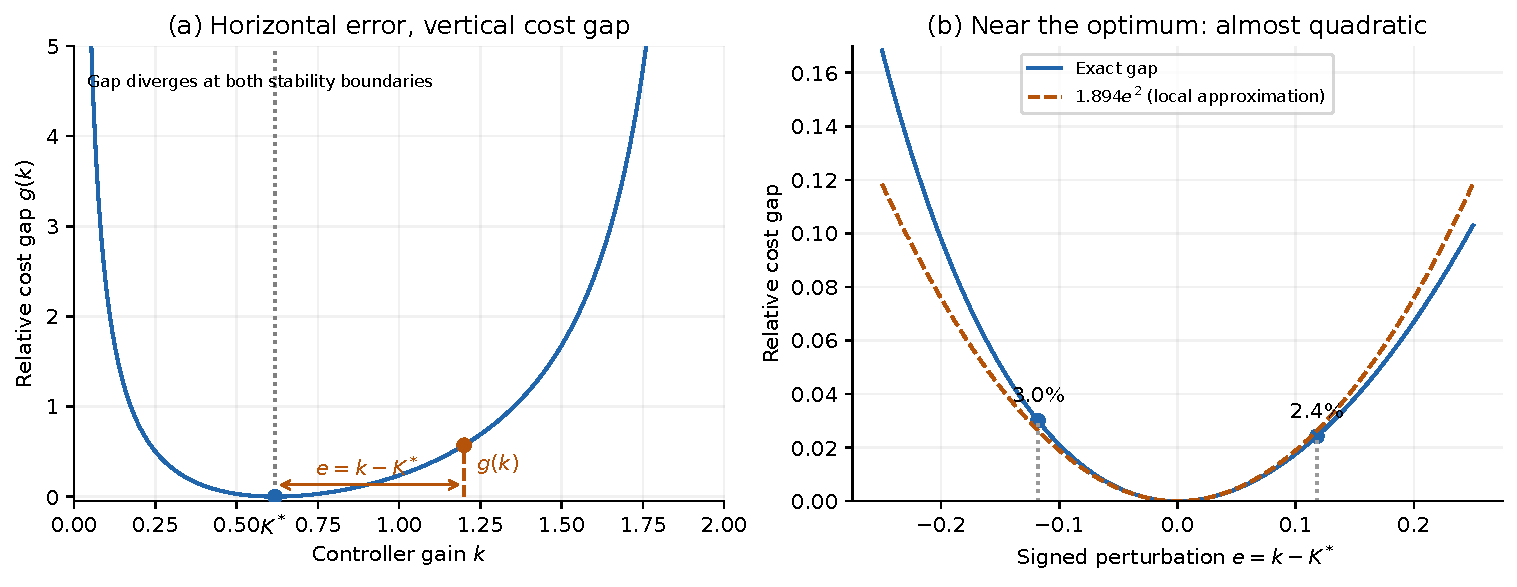
\includegraphics[width=\textwidth]{gap-geometry.pdf}
  \caption{The scalar LQR gap. Left: a perturbation is a horizontal displacement
    from $K^*$; its cost gap is the height of the curve. The vertical axis is
    truncated because the gap diverges at $k=0$ and $k=2$.
    Right: the exact gap and its quadratic approximation near the optimum.
    Equal perturbation magnitudes of $0.118$ give different gaps on opposite
    sides: approximately $3.0\%$ below and $2.4\%$ above the optimal gain.
    A relative gap of $0.03$ means a cost $3\%$ above the optimum.}
  \label{fig:gap-geometry}
\end{figure}

\emph{A small perturbation gives a small gap.} Between zero and two the cost is a ratio of
polynomials with a nonzero denominator, so the gap is continuous there. Continuity at the optimal
gain, where the gap is zero, says exactly:
\[
  \forall \varepsilon > 0 \ \exists \delta > 0 : \quad
  |k - K^*| < \delta \ \Longrightarrow\ g(k) < \varepsilon .
\]

\emph{A small gap gives a small perturbation.} This holds because the optimal gain is the unique
minimizer:
\[
  \forall \eta > 0 \ \exists \varepsilon > 0 : \quad
  g(k) < \varepsilon \ \Longrightarrow\ |k - K^*| < \eta .
\]
To find such an $\varepsilon$, take the smaller of the two gaps at distance $\eta$ from the optimal
gain, for $\eta$ smaller than the optimal gain:
\[
  \varepsilon = \min\big\{\, g(K^* - \eta),\ g(K^* + \eta) \,\big\} > 0 .
\]
The gap decreases toward the optimal gain from the left and increases away from it on the right, so
every gain at distance $\eta$ or more has a gap of at least $\varepsilon$. A gap below
$\varepsilon$ therefore forces a distance below $\eta$.

Applying the two facts along the sequence of gains of a run: once the learning curve stays below
$\varepsilon$, the perturbation stays below $\eta$, and once the perturbation stays below $\delta$,
the learning curve stays below $\varepsilon$. This gives
\[
  g_X(N) \to 0 \iff k_X(N) \to K^* \iff e_X(N) \to 0 .
\]
Both facts hold for any continuous gap with a unique minimum, not only for this example.

\paragraph{Expansion near the optimal gain.} Differentiate the identity $f = J h$ twice and evaluate
at the optimal gain, where the first derivative of the cost vanishes:
\[
  f'' = J'' h + 2 J' h' + J h''
  \quad\Longrightarrow\quad
  J''(K^*) = \frac{f''(K^*) - J^* h''(K^*)}{h(K^*)} = \frac{2 + 2J^*}{h(K^*)} .
\]
Using the Riccati identity for the optimal gain to simplify the denominator:
\begin{gather*}
  (K^*)^2 = 1 - K^* \ \Longrightarrow\ h(K^*) = 2K^* - (K^*)^2 = 3K^* - 1 = \frac{3\sqrt{5} - 5}{2}, \\
  J''(K^*) = \frac{2\,(3 + \sqrt{5})}{3\sqrt{5} - 5} = \frac{7\sqrt{5} + 15}{5} \approx 6.130 .
\end{gather*}
Taylor's theorem at the minimum, where the first derivative vanishes, gives the gap to second order:
\begin{gather*}
  g(K^* + e) = \frac{J(K^* + e)}{J^*} - 1 = \frac{J''(K^*)}{2J^*}\, e^2 + O(e^3), \\
  \frac{J''(K^*)}{2J^*} = \frac{7\sqrt{5} + 15}{5\,(1 + \sqrt{5})} = 1 + \frac{2}{\sqrt{5}} \approx 1.894 .
\end{gather*}
The higher-order terms were bounded numerically on a neighbourhood of the optimal gain:
\[
  1.758\, e^2 \le g(K^* + e) \le 2.108\, e^2 \qquad \text{for } |e| \le 0.1 .
\]
The bounds give explicit choices in the two facts. For the first, the upper bound controls the gap
by the perturbation; for the second, the lower bound and the monotonicity above control the
perturbation by the gap:
\[
  |e| < \delta = \sqrt{\varepsilon / 2.108} \le 0.1
  \ \Longrightarrow\ g(K^* + e) \le 2.108\, e^2 < 2.108\, \delta^2 = \varepsilon ,
\]
\[
  \eta \le 0.1, \ \varepsilon = 1.758\, \eta^2: \quad
  |e| \ge \eta \ \Longrightarrow\ g(K^* + e) \ge \min\big\{ g(K^* - \eta), g(K^* + \eta) \big\}
  \ge 1.758\, \eta^2 = \varepsilon .
\]
The two observations below come from evaluating the cost directly, using the simplification above:
\begin{gather*}
  g(0.5) = K^* \cdot \frac{1.25}{0.75} - 1 \approx 0.030, \qquad
  g(0.736) = K^* \cdot \frac{1.5417}{0.9303} - 1 \approx 0.024, \\
  0.5 - K^* \approx -0.118, \qquad 0.736 - K^* \approx +0.118 .
\end{gather*}
\begin{itemize}
  \item \textbf{Observation 1.} A gain about 19\% below the optimum has a gap of only about 3\%: the
    gap is quadratic in the perturbation.
  \item \textbf{Observation 2.} Undershooting and overshooting the optimal gain by the same amount,
    0.118, give gaps of 0.030 and 0.024: undershooting costs more, because the left wall is closer.
\end{itemize}

\paragraph{Limits.} If the gain of a run settles at a stabilizing value, continuity carries the limit
through the gap, so the floor of the learning curve is the gap at the limit gain:
\[
  k_X(N) \to k_{X,\infty} \in (0, 2) \ \Longrightarrow\ g_X(N) \to g\big(k_{X,\infty}\big).
\]

\paragraph{Ordering.} The learning curves of the three algorithms may be ordered at every iteration,
or only after some iteration:
\[
  g_A(N) \le g_B(N) \le g_C(N) \quad \forall N, \qquad
  \exists\, N_0 : \ g_A(N) \le g_B(N) \le g_C(N) \quad \forall N \ge N_0 .
\]
The smallest such iteration is the crossing time. Near the optimal gain the gap is, to leading
order, an increasing function of the size of the perturbation, so the ordering of the curves follows
the ordering of the perturbations. If the perturbations decay like power laws, the ratio of two of
them shows which one wins eventually and when they cross:
\[
  |e_X(N)| \approx \kappa_X N^{-\beta_X}
  \ \Longrightarrow\
  \frac{|e_X(N)|}{|e_Y(N)|} \approx \frac{\kappa_X}{\kappa_Y}\, N^{-(\beta_X - \beta_Y)} \to 0
  \quad \text{if } \beta_X > \beta_Y ,
\]
\[
  \frac{\kappa_X}{\kappa_Y}\, N^{-(\beta_X - \beta_Y)} = 1
  \iff N = N_{XY} = \left(\frac{\kappa_X}{\kappa_Y}\right)^{1/(\beta_X - \beta_Y)} .
\]
So the faster-decaying algorithm is eventually below; if it starts above, it crosses below at the
iteration shown.

\begin{figure}[H]
  \centering
  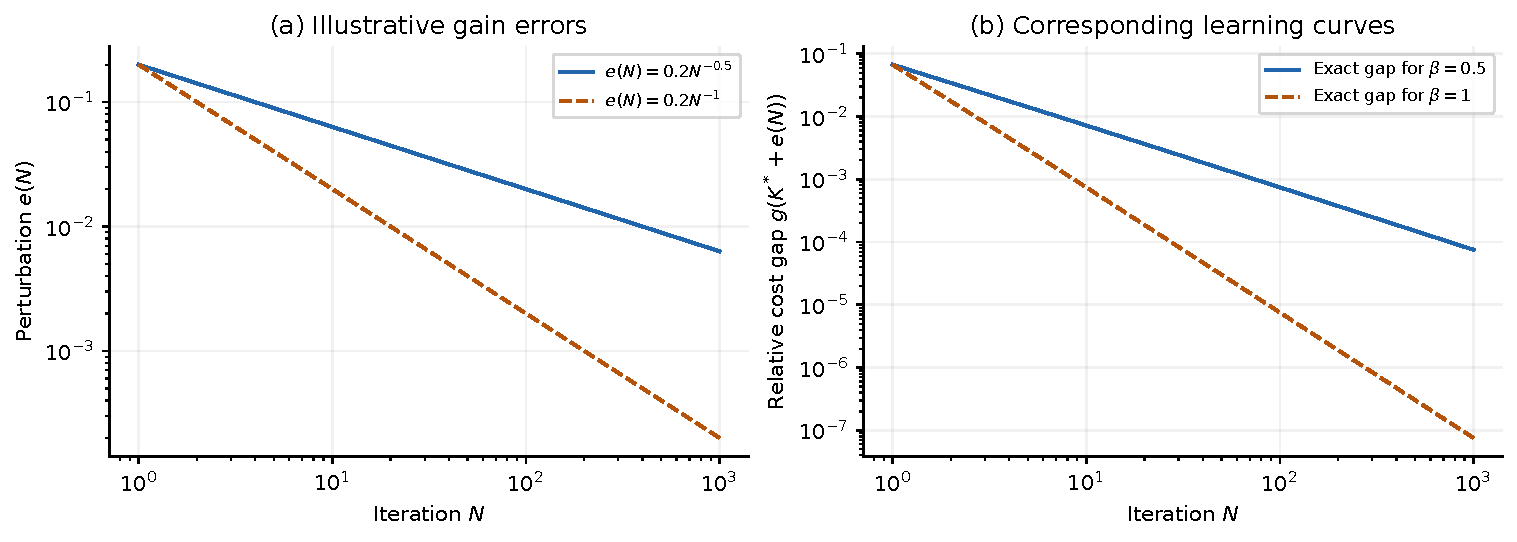
\includegraphics[width=\textwidth]{perturbation-learning-curves.pdf}
  \caption{How shrinking perturbations become shrinking learning curves.
    These are constructed examples, not measured RL training runs.
    Left: two positive perturbations $e(N)=0.2N^{-\beta}$ with
    $\beta=1/2$ and $\beta=1$. Right: their gaps evaluated with the exact
    scalar cost formula. Both axes use logarithmic scales.
    Near the optimum, $g\approx 1.894 e^2$, so a perturbation decaying as
    $N^{-\beta}$ gives a gap decaying approximately as $N^{-2\beta}$:
    halving a small perturbation approximately quarters the gap.}
  \label{fig:perturbation-learning-curves}
\end{figure}

%----------------------------------------------------------------------------------------------------
\section{Many seeds}
\label{sec:seeds}

A seed is a random number. All the randomness in one training run, the initial parameters, the
exploration noise and any noise in the environment, is generated from it, so once the seed is picked
the run is deterministic. The set of seeds $\Omega$ is a set of random numbers; in code it is a
finite set of integers, which can be pictured as points on a line:
\[
  \Omega = \{\, 0, 1, 2, \dots, 2^{32} - 1 \,\} \subset \mathbb{R}, \qquad \omega \in \Omega .
\]
Picking a seed is drawing a point from this line, and each point gives one learning curve. Over all
of $\Omega$, an algorithm therefore produces a collection of learning curves, one per seed, and the
analysis of the algorithm is the analysis of this collection: its average, its spread, its bounds and
where it settles. The question of the notes is whether, as training time increases, the ordering of
Section~\ref{sec:onerun} holds for every seed on this line.

The curves are bounded below, because no gain does better than the optimum:
\[
  J(k) \ge J^* \quad\Longrightarrow\quad g_X(\omega, N) \ge 0 \quad \text{for every seed and iteration} .
\]
They are also bounded above whenever the gains of the runs stay in a closed interval inside the
stability region, because the gap is continuous there and a continuous function is bounded on a
closed interval. So the expected curve below is finite once the runs that leave the stability region
are counted separately.

\paragraph{Functions.} Seeds are drawn uniformly from the set of integer seeds, and the gain and
learning curve become functions of the seed as well as the iteration:
\[
  \omega \in \Omega, \qquad P(\omega) = 2^{-32},
\]
\begin{align*}
  k_X &: \Omega \times \mathbb{N} \to \mathbb{R}, &
    k_X(\omega, N) &= \text{gain after } N \text{ iterations with seed } \omega, \\
  g_X &: \Omega \times \mathbb{N} \to [0, \infty], &
    g_X(\omega, N) &= g\big(k_X(\omega, N)\big).
\end{align*}
Fixing $\omega$ recovers Section~\ref{sec:onerun}.

\paragraph{Expected and estimated curves.} Over all seeds, and over the $M$ seeds run:
\[
  \bar g_X(N) = \sum_{\omega \in \Omega} P(\omega)\, g\big(k_X(\omega, N)\big), \qquad
  \hat g_X(N) = \frac{1}{M} \sum_{j=1}^{M} g\big(k_X(\omega_j, N)\big).
\]
The seeds are independent, so the variance of an average of $M$ curves is the variance of one curve
divided by $M$:
\begin{gather*}
  \operatorname{Var}\big[\hat g_X(N)\big] = \frac{1}{M^2} \sum_{j=1}^{M}
    \operatorname{Var}\big[g_X(\omega_j, N)\big] = \frac{\sigma_X(N)^2}{M}, \\
  \operatorname{SE}\big[\hat g_X(N)\big] = \frac{\sigma_X(N)}{\sqrt{M}}, \qquad
  \sigma_X(N)^2 = \operatorname{Var}\big[g_X(\cdot, N)\big].
\end{gather*}
Runs whose gain does not stabilize the system are counted as failures and excluded from the
averages.

\paragraph{Bias and variance.} Averaging the expansion near the optimal gain over seeds gives
\begin{gather*}
  \bar g_X(N) \approx \Big(1 + \frac{2}{\sqrt{5}}\Big)\, \mathbb{E}\big[e_X(\cdot, N)^2\big], \\
  \mathbb{E}[e^2] = \big(\mathbb{E}[e]\big)^2 + \operatorname{Var}[e], \qquad
  \mathbb{E}[e] = \mathbb{E}[k] - K^*, \qquad \operatorname{Var}[e] = \operatorname{Var}[k],
\end{gather*}
where the middle identity is the definition of variance rearranged, and the last two hold because
the perturbation is the gain shifted by a constant. Together:
\[
  \bar g_X(N) \approx \Big(1 + \frac{2}{\sqrt{5}}\Big)\Big[\big(\mathbb{E}[k_X(\cdot, N)] - K^*\big)^2
  + \operatorname{Var}\big[k_X(\cdot, N)\big]\Big].
\]
\begin{itemize}
  \item \textbf{Observation 3.} The expected gap splits into squared bias (settling at the wrong gain
    on average) and variance (inconsistency across seeds).
\end{itemize}

\paragraph{Ordering across seeds.} From strongest to weakest:
\[
  \max_{\omega} g_A(\omega, N) \le \min_{\omega'} g_B(\omega', N), \qquad
  \bar g_A(N) \le \bar g_B(N), \qquad
  \lim_{N \to \infty} \bar g_A(N) \le \lim_{N \to \infty} \bar g_B(N),
\]
that is, band separation, expected-curve ordering, and floor ordering. Each implies the next. Band
separation places every run of $A$ below every run of $B$, so averaging over both sets of seeds keeps
the inequality; taking limits keeps it again:
\begin{gather*}
  g_A(\omega, N) \le \max_{\omega} g_A(\omega, N) \le \min_{\omega'} g_B(\omega', N)
    \le g_B(\omega', N) \\
  \Longrightarrow\ \bar g_A(N) \le \bar g_B(N)
  \ \Longrightarrow\ \lim_{N \to \infty} \bar g_A(N) \le \lim_{N \to \infty} \bar g_B(N).
\end{gather*}

The converses, the same implications read backwards, fail. Each reversed arrow fails for its own
reason, shown by one counterexample.

\emph{Floor ordering does not imply expected-curve ordering.} A floor depends only on the tail of a
curve, so two curves can end in one order after crossing early on:
\[
  \bar g_A(N) = 0.1 + \frac{10}{N}, \qquad \bar g_B(N) = 0.2 + \frac{1}{N}: \qquad
  \lim_{N \to \infty} \bar g_A = 0.1 < 0.2 = \lim_{N \to \infty} \bar g_B ,
\]
\[
  \bar g_A(N) > \bar g_B(N) \iff 0.1 + \frac{10}{N} > 0.2 + \frac{1}{N}
  \iff \frac{9}{N} > 0.1 \iff N < 90 .
\]
Algorithm $A$ starts much worse and overtakes $B$ only after 90 iterations; the floors alone hide
this.

\emph{Expected-curve ordering does not imply band separation.} An average can be ordered while
individual runs are not. Suppose two seeds of each algorithm give these gaps at some iteration:
\begin{center}
  \begin{tabular}{lccc}
    \toprule
      & Seed 1 & Seed 2 & Average \\
    \midrule
    $A$ & 0.01 & 0.05 & 0.03 \\
    $B$ & 0.02 & 0.06 & 0.04 \\
    \bottomrule
  \end{tabular}
\end{center}
The averages are ordered, 0.03 below 0.04, but the worst run of $A$, 0.05, is above the best run of
$B$, 0.02. The two sets of runs overlap, so not every run of $A$ beats every run of $B$.

For an experiment, this means each claim must be checked on its own. Ordered floors say nothing about
early training, and ordered averages say nothing about individual runs; only band separation supports
a statement about every run at every iteration.

%----------------------------------------------------------------------------------------------------
\section{A possible experiment}

\begin{itemize}
  \item Train $A$, $B$ and $C$ on the scalar system with reward $r_t = -(x_t^2 + u_t^2)$ and linear
    policies $u = -kx$; a neural-network variant is evaluated by simulation.
  \item Keep tuning seeds separate from evaluation seeds.
  \item Record $k_X(\omega, N)$ and $g_X(\omega, N)$ at checkpoints; count gains outside $(0, 2)$ as
    failures.
  \item Report $\hat g_X$ with confidence bands, the floors, the bias and variance of the final gains,
    the crossing times, and which ordering of Section~\ref{sec:seeds} holds.
\end{itemize}

%----------------------------------------------------------------------------------------------------
\section{Limitations}
\label{sec:limitations}

\begin{itemize}
  \item \textbf{Discounting.} $K^*$ and $J^*$ depend on $\gamma$; compute them with the agents'
    $\gamma$.
  \item \textbf{Noise.} $J$ becomes an expectation; in the scalar case the shape of $g$ is unchanged.
  \item \textbf{Linear policies.} They give the agent the form of the solution; the neural variant
    tests the realistic case.
  \item \textbf{Locality.} The expansion holds only near $K^*$.
  \item \textbf{Higher dimensions.} $K$ becomes a matrix and the expansion involves a Hessian.
  \item \textbf{SAC.} Evaluate it by its mean action to avoid the effect of the entropy bonus.
\end{itemize}

%----------------------------------------------------------------------------------------------------
\appendix

\section{Proximal Policy Optimization (PPO)}
\label{app:ppo}

PPO (Schulman et al.\ 2017) is an on-policy actor-critic algorithm. It alternates between collecting
data with the current policy and taking several gradient steps on a clipped objective that keeps the
new policy close to the one that collected the data.

\paragraph{Components.} A stochastic policy with parameters $\theta$ and a value function with
parameters $\phi$:
\[
  \pi_\theta(u \mid x), \qquad V_\phi(x) .
\]

\paragraph{Probability ratio.} How much more or less likely the new policy makes an action than the
policy that collected it:
\[
  \rho_t(\theta) = \frac{\pi_\theta(u_t \mid x_t)}{\pi_{\theta_{\mathrm{old}}}(u_t \mid x_t)} .
\]

\paragraph{Advantage estimate.} The temporal-difference errors of the value function, combined by
generalized advantage estimation (Schulman et al.\ 2016) with discount $\gamma$ and weight $\lambda$:
\[
  \delta_t = r_t + \gamma V_\phi(x_{t+1}) - V_\phi(x_t), \qquad
  \hat A_t = \sum_{l=0}^{T - t - 1} (\gamma \lambda)^l\, \delta_{t+l}, \qquad
  \hat R_t = \hat A_t + V_\phi(x_t) .
\]

\paragraph{Clipped policy objective.} With clipping parameter $\varepsilon_{\mathrm{clip}}$:
\[
  L^{\mathrm{CLIP}}(\theta) = \hat{\mathbb{E}}_t\Big[\min\big(\rho_t(\theta)\, \hat A_t,\
  \operatorname{clip}\big(\rho_t(\theta),\, 1 - \varepsilon_{\mathrm{clip}},\,
  1 + \varepsilon_{\mathrm{clip}}\big)\, \hat A_t\big)\Big].
\]

\paragraph{Value loss and entropy bonus.}
\[
  L^{V}(\phi) = \hat{\mathbb{E}}_t\Big[\big(V_\phi(x_t) - \hat R_t\big)^2\Big], \qquad
  S[\pi_\theta](x_t) = -\int \pi_\theta(u \mid x_t) \log \pi_\theta(u \mid x_t)\, du .
\]

\paragraph{Combined objective.} Maximized with weights $c_1$ and $c_2$:
\[
  L(\theta, \phi) = \hat{\mathbb{E}}_t\Big[ L^{\mathrm{CLIP}}_t(\theta) - c_1 L^{V}_t(\phi)
  + c_2\, S[\pi_\theta](x_t) \Big].
\]

\paragraph{Algorithm.}
\begin{enumerate}
  \item Initialize the policy parameters $\theta$ and the value parameters $\phi$.
  \item For each iteration:
    \begin{enumerate}
      \item Set the data-collecting policy to the current one, $\theta_{\mathrm{old}} \leftarrow \theta$.
      \item Run the policy for $T$ time steps (in one or more parallel environments) and store the
        states, controls and rewards.
      \item Compute the temporal-difference errors, the advantage estimates and the return targets
        from the stored data.
      \item For $E$ epochs, split the data into minibatches and, on each minibatch, take a gradient
        ascent step on the combined objective with respect to $\theta$ and $\phi$.
    \end{enumerate}
  \item Return the final policy.
\end{enumerate}

%----------------------------------------------------------------------------------------------------
\section{A new test of ideas: PPO with one fixed seed}
\label{sec:ppo-fixed-seed}

This appendix specializes the gap and perturbation analysis of Section~\ref{sec:onerun}
to one fixed seed of PPO, introduced in Appendix~\ref{app:ppo}.

Fix a seed $\omega_0$. For the scalar system $a=b=q=r=x_0=1$, let
$k_N := k_{\mathrm{PPO}}(\omega_0,N)$ be the gain of PPO's linear mean policy
at iteration $N$. Evaluate the deterministic mean action $u_t=-k_Nx_t$.

\paragraph{The gap and perturbation, expanded.}
\begin{align*}
  K^* &= \frac{\sqrt{5}-1}{2}, & J^* &= \frac{1+\sqrt{5}}{2}, \\
  e_{\mathrm{PPO}}(\omega_0,N)
    &= k_N-\frac{\sqrt{5}-1}{2}, &
  x_t &= (1-k_N)^t .
\end{align*}
For $0<k_N<2$,
\begin{align*}
  J(k_N)
    &= \sum_{t=0}^{\infty}\big(x_t^2+(-k_Nx_t)^2\big) \\
    &= \sum_{t=0}^{\infty}(1+k_N^2)(1-k_N)^{2t} \\
    &= \frac{1+k_N^2}{1-(1-k_N)^2}
     = \frac{1+k_N^2}{k_N(2-k_N)}, \\
  g_{\mathrm{PPO}}(\omega_0,N)
    &= \frac{\dfrac{1+k_N^2}{k_N(2-k_N)}-\dfrac{1+\sqrt{5}}{2}}
             {\dfrac{1+\sqrt{5}}{2}} \\
    &= \frac{(\sqrt{5}-1)(1+k_N^2)}{2k_N(2-k_N)}-1 \\
    &= \frac{(\sqrt{5}+1)k_N^2-4k_N+(\sqrt{5}-1)}{2k_N(2-k_N)} \\
    &= \frac{(\sqrt{5}+1)\left(k_N-\dfrac{\sqrt{5}-1}{2}\right)^2}
             {2k_N(2-k_N)} .
\end{align*}
For $k_N\notin(0,2)$, $J(k_N)=g_{\mathrm{PPO}}(\omega_0,N)=+\infty$.
Writing $e_N:=e_{\mathrm{PPO}}(\omega_0,N)$, the definition of the perturbation gives
\[
  e_N=k_N-K^*=k_N-\frac{\sqrt{5}-1}{2}
  \quad\Longrightarrow\quad
  k_N=\frac{\sqrt{5}-1}{2}+e_N.
\]
The other factor in the denominator becomes
\[
  2-k_N=2-\left(\frac{\sqrt{5}-1}{2}+e_N\right)
  =\frac{4-\sqrt{5}+1}{2}-e_N
  =\frac{5-\sqrt{5}}{2}-e_N.
\]
The interval for $e_N$ comes from the stability condition, not from a bound on PPO's
updates. For the fixed gain at iteration $N$, the closed-loop dynamics are
$x_{t+1}=(1-k_N)x_t$, so stability requires
\[
  |1-k_N|<1
  \quad\Longleftrightarrow\quad -1<1-k_N<1
  \quad\Longleftrightarrow\quad 0<k_N<2.
\]
Subtracting $K^*$ from all three parts and substituting $e_N=k_N-K^*$ gives
\begin{align*}
  0<k_N<2
  &\quad\Longleftrightarrow\quad -K^*<k_N-K^*<2-K^* \\
  &\quad\Longleftrightarrow\quad
    -\frac{\sqrt{5}-1}{2}<e_N<2-\frac{\sqrt{5}-1}{2} \\
  &\quad\Longleftrightarrow\quad
    -\frac{\sqrt{5}-1}{2}<e_N<\frac{5-\sqrt{5}}{2}.
\end{align*}
Numerically, this is $-0.618\ldots<e_N<1.382\ldots$. It is exactly the stability
interval expressed in terms of the perturbation; PPO is not guaranteed to keep
its gains inside this interval. At either endpoint or outside it, the cost and
gap are infinite for the initial state $x_0=1$.

Substituting the expressions for $k_N$ and $2-k_N$ into the factored gap above
gives the exact expression on this interval:
\[
  g_{\mathrm{PPO}}(\omega_0,N)
  = \frac{(\sqrt{5}+1)e_N^2}
    {2\left(\dfrac{\sqrt{5}-1}{2}+e_N\right)
       \left(\dfrac{5-\sqrt{5}}{2}-e_N\right)},
  \qquad
  -\frac{\sqrt{5}-1}{2}<e_N<\frac{5-\sqrt{5}}{2}.
\]

\paragraph{Proposition 1: a small perturbation gives a small gap.}
For every $\varepsilon>0$, there exists $\delta>0$ such that, for every $N$,
\[
  \left|k_N-\frac{\sqrt{5}-1}{2}\right|<\delta
  \quad\Longrightarrow\quad
  \frac{(\sqrt{5}-1)(1+k_N^2)}{2k_N(2-k_N)}-1<\varepsilon .
\]
One explicit choice is
\[
  \delta=\min\left\{0.1,\sqrt{\frac{\varepsilon}{2.108}}\right\}.
\]

\paragraph{Proposition 2: a small gap gives a small perturbation.}
For every $\eta>0$, there exists $\varepsilon>0$ such that, for every $N$
with $0<k_N<2$,
\[
  \frac{(\sqrt{5}-1)(1+k_N^2)}{2k_N(2-k_N)}-1<\varepsilon
  \quad\Longrightarrow\quad
  \left|k_N-\frac{\sqrt{5}-1}{2}\right|<\eta .
\]
For $0<\eta<(\sqrt{5}-1)/2$, an explicit choice is
\[
  \varepsilon=\min\left\{
  \frac{(\sqrt{5}+1)\eta^2}
       {2\left(\dfrac{\sqrt{5}-1}{2}-\eta\right)
          \left(\dfrac{5-\sqrt{5}}{2}+\eta\right)},\quad
  \frac{(\sqrt{5}+1)\eta^2}
       {2\left(\dfrac{\sqrt{5}-1}{2}+\eta\right)
          \left(\dfrac{5-\sqrt{5}}{2}-\eta\right)}
  \right\}.
\]

\paragraph{Proposition 3: convergence of the gap and perturbation.}
For a sequence of stabilizing gains,
\begin{gather*}
  \lim_{N\to\infty}
  \left[\frac{(\sqrt{5}-1)(1+k_N^2)}{2k_N(2-k_N)}-1\right]=0
  \\
  \Longleftrightarrow\quad
  \lim_{N\to\infty}k_N=\frac{\sqrt{5}-1}{2}
  \quad\Longleftrightarrow\quad
  \lim_{N\to\infty}\left(k_N-\frac{\sqrt{5}-1}{2}\right)=0 .
\end{gather*}

\paragraph{Proposition 4: the local quadratic relation.}
As $k_N\to(\sqrt{5}-1)/2$,
\begin{align*}
  \frac{(\sqrt{5}-1)(1+k_N^2)}{2k_N(2-k_N)}-1
  &=\left(1+\frac{2}{\sqrt{5}}\right)
      \left(k_N-\frac{\sqrt{5}-1}{2}\right)^2 \\
  &\quad+O\!\left(\left|k_N-\frac{\sqrt{5}-1}{2}\right|^3\right).
\end{align*}
For $\left|k_N-(\sqrt{5}-1)/2\right|\le0.1$,
\[
  1.758\left(k_N-\frac{\sqrt{5}-1}{2}\right)^2
  \le \frac{(\sqrt{5}-1)(1+k_N^2)}{2k_N(2-k_N)}-1
  \le 2.108\left(k_N-\frac{\sqrt{5}-1}{2}\right)^2 .
\]

%----------------------------------------------------------------------------------------------------
\section*{References}

\begin{itemize}
  \item Agarwal, R., Schwarzer, M., Castro, P.~S., Courville, A., and Bellemare, M.~G. (2021). Deep
    reinforcement learning at the edge of the statistical precipice. \emph{NeurIPS 2021}.
  \item Agyei, K., Sarhadi, P., and Polani, D. (2025).
    \href{https://arxiv.org/html/2507.08196}{Deep reinforcement learning in applied control:
    Challenges, analysis, and insights}. arXiv:2507.08196.
  \item Fazel, M., Ge, R., Kakade, S.~M., and Mesbahi, M. (2018).
    \href{https://proceedings.mlr.press/v80/fazel18a.html}{Global convergence of policy gradient
    methods for the linear quadratic regulator}. \emph{ICML 2018}.
  \item Henderson, P., Islam, R., Bachman, P., Pineau, J., Precup, D., and Meger, D. (2018). Deep
    reinforcement learning that matters. \emph{AAAI 2018}.
  \item Mania, H., Guy, A., and Recht, B. (2018).
    \href{https://arxiv.org/pdf/1803.07055}{Simple random search provides a competitive approach to
    reinforcement learning}. arXiv:1803.07055.
  \item Recht, B. (2019). \href{https://arxiv.org/pdf/1806.09460}{A tour of reinforcement learning:
    The view from continuous control}. \emph{Annual Review of Control, Robotics, and Autonomous
    Systems}. arXiv:1806.09460.
  \item Schulman, J., Moritz, P., Levine, S., Jordan, M., and Abbeel, P. (2016). High-dimensional
    continuous control using generalized advantage estimation. \emph{ICLR 2016}. arXiv:1506.02438.
  \item Schulman, J., Wolski, F., Dhariwal, P., Radford, A., and Klimov, O. (2017). Proximal policy
    optimization algorithms. arXiv:1707.06347.
  \item Tu, S., and Recht, B. (2019). \href{https://arxiv.org/pdf/1812.03565}{The gap between
    model-based and model-free methods on the linear quadratic regulator: An asymptotic viewpoint}.
    arXiv:1812.03565.
\end{itemize}

\end{document}
